%% \startreport{A/B Statistics}
%% \reportauthor{Some Jokers}
\documentclass[12pt]{report}
\usepackage{hyperref}
\usepackage{amsmath}
\usepackage{graphicx}
\newcommand{\be}{\begin{enumerate}} %% same as ramesh_abbr
\newcommand{\ee}{\end{enumerate}} %% same as ramesh_abbr
\newcommand{\beq}{\begin{equation}} %% new, no conflict
\newcommand{\eeq}{\end{equation}} %% new, no conflict
\newcommand{\bdm}{\begin{displaymath}} %% new, no conflict
\newcommand{\edm}{\end{displaymath}} %% new, no conflict
\newcommand{\bi}{\begin{itemize}} %% same as ramesh_abbr
\newcommand{\ei}{\end{itemize}} %% same as ramesh_abbr
\newcommand{\TBC}{\framebox{\textbf{TO BE COMPLETED}}} %% same as ramesh_abbr
\newcommand{\reals}{{\rm I\! R}} %% new, no conflict

\begin{document}

\title{A or B? A Bayesian Approach for Binary outcome tests}
\author{Ramesh Subramonian, Ranjeet S. Tate, Michael Shire, Abhinav Singh}
\date{}
\maketitle

\section{Parametric Approach}

Instead of calculating the above integrals for the Bayesian
probability distribution, one could try and approximate the required
probability \(\Pi[M(p_A, p_B)>0]\) by taking a parametric
approach. Consider again the one-dimensional case. Since the beta
distribution is "bell shaped", the parametric approach suggests
approximating the beta distribution as a normal distribution with
suitable mean and variance (the parameters). If we are interested in
simply knowing whether \(x-x_c>0\), we can calculate the corresponding
\bdm
z = \frac{<x>-x_c}{SE(<x>)}
\edm
and use the normal \(z\rightarrow p\) calculators or
the cumulative function of
the normal distribution to calculate the credibility.

To calculate the probability that \(M(x)>0\), one can
(quite incorrectly, since non-linear transformations will not preserve
normality) assume that the \(\{M(x)\}\) are also normally
distributed. We can calculate the mean \(<M(x)>\) and the
Standard Error of the mean \(SE(<M(x)>\) of the function using
well-known approximations and proceed as before to compute \(z\) and
\(p\). Generalizing to a function \(M(x,y)\) on 2D probability space:
\beq
\begin{split}
  <M> &\approx M(<x>,<y>)\\
  var(M) &\approx \left(\frac{\partial M}{\partial x}\right)^2\cdot var(x)
  + \left(\frac{\partial M}{\partial y}\right)^2\cdot var(y)
\end{split}
\eeq
where we are assuming that \(x\) and \(y\) are independent.

What parameters should one use for the normal approximation? If we were
taking a frequentist approach we would use \(\mu =m/n\)
and \(variance = \frac{\mu\cdot(1-\mu)}{n}\), however, these are
not the correct parameters to use for approximations to the beta
distribution. The above values are the mean and variance of the mean
for the original
binary valued distribution. What we are interested in is the normal
approximation to the Bayesian posterior distribution corresponding to the
experimental outcome \( (n,m) \), which is the beta distribution. Recall that
the mean and variance for the beta distribution are
\beq
\begin{split}
  \mu' &= \frac{m+1}{n+2}\\
  variance &= \frac{\mu'\cdot (1-\mu')}{n+3}
\end{split}
\eeq

How do we compare the normal approximation to the beta distribution?
The values for the distributions themselves are not particularly useful,
one is much more
interested in the quantiles or the cumulative function. So we
should compare the cumulative functions of the beta distribution and
of the normal distribution over the range of \(p\),
\begin{figure}[ht!]
\centering
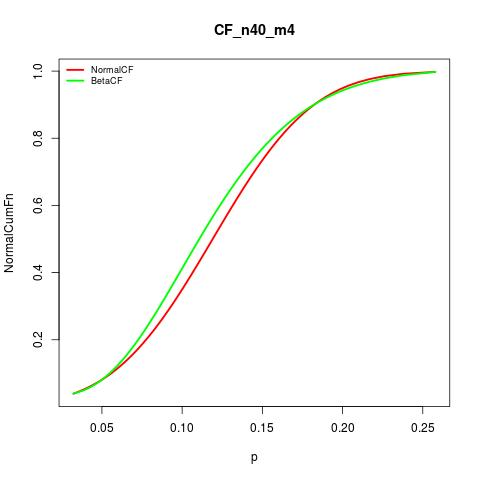
\includegraphics[width=90mm]{CF_n40_m4}
\caption{Normal and Beta Cumulative Functions \label{fig:normal_vs_betaCF}}
\end{figure}
and see whether they
are close enough by some metric. See Fig. \ref{fig:normal_vs_betaCF} in
which we've plotted the cumulative functions of both the normal and beta
distributions for \(n=40, m=4\).

What metric should we use to compare the cumulative functions?
Since the cumulative functions
are probabilities, we will run into the same issues we had with the
difference and lift metrics.  So the metric we will use is the relative odds
ratio.  Specifically, we will calculate {\it abs(log(relative odds ratio))},
and see whether this
remains below some threshold for tolerance about 0. If our tolerance for the
relative error
in the values of the cumulative functions
is approximately 10\%, then we want the abs(log(relative odds ratio)) to be
bounded by 0.1 since \({\tt lim}_{x\rightarrow 0}log(1+x)=x\).
\begin{figure}[ht!]
\centering
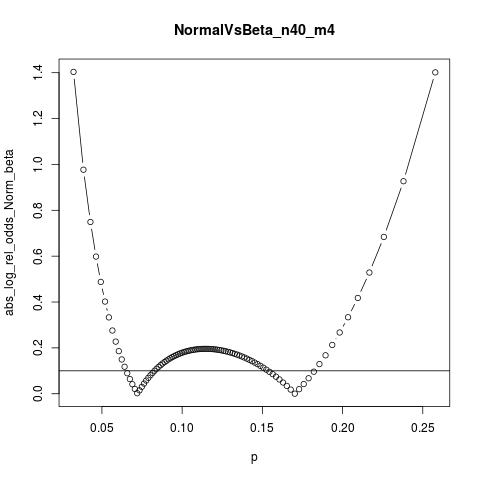
\includegraphics[width=90mm]{NormalVsBeta_n40_m4}
\caption{Comparing Cumulative Functions: Normal {\em not} a tolerable
approximation to \(\beta\) \label{fig:NormalVsBeta_40_4}}
\end{figure}
In Fig. \ref{fig:NormalVsBeta_40_4} we plot the absolute value of the log
of the odds ratio for the cumulative functions of the Normal and Beta
distributions for \(n=40, m=4\), the same data as before. We see that there is
no reasonable continuous range in which the normal distribution is a
good estimate of the beta distribution for such statistically small data.

Is there a regime in which the normal distribution {\em is} a good
approximation (to within 10\% of the odds) to the beta distribution? Yes,
consider the case when \(n=400, m=20\).
\begin{figure}[ht!]
\centering
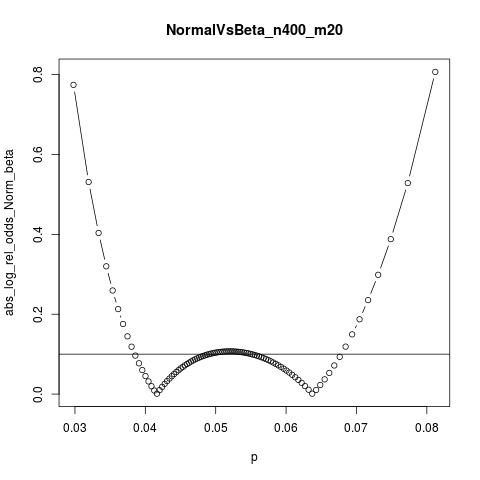
\includegraphics[width=90mm]{NormalVsBeta_n400_m20}
\caption{Comparing Cumulative Functions: Range in which Normal is a
tolerable approximation to \(\beta\) \label{fig:NormalVsBeta_400_20}}
\end{figure}
The error metric is shown in Fig. \ref{fig:NormalVsBeta_400_20}.
We see that the approximation is within the tolerance of 10\% for
\(p\in[0.038,0.068]\). From the cumulative function for beta,
\begin{figure}[ht!]
\centering
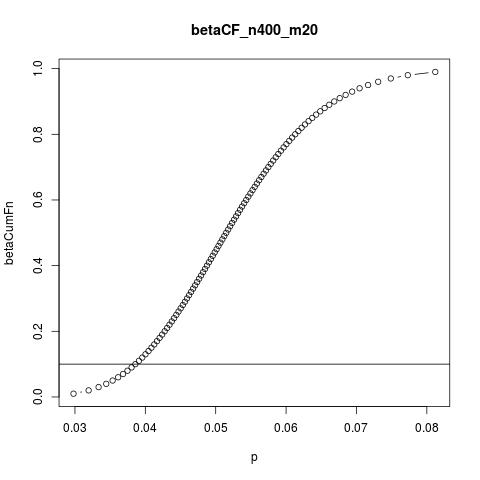
\includegraphics[width=90mm]{betaCF_n400_m20}
\caption{Percentile Range in which Normal is a
tolerable approximation to \(\beta\)  \label{fig:betaCF_400_20}}
\end{figure}
shown in Fig. \ref{fig:betaCF_400_20},
one can read off the corresponding credibility range, which is \([10\%,90\%]\).
90\% is close to the minimum credibility one should require for a
business decision, so for any credibility of interest \(>90\%\) the
normal distribution is {\em not} a tolerable
approximation to the beta distribution.

From considerations like the above, we can state as a rule of thumb
that the normal
is a tolerable approximation to the beta distribution when \(n>100\)
and \(m>20\).

For a metric comparing the two Bayesian probabilities the situation is worse
due to the approximations involved in the nonlinearities as well as the fact
that any such metric ``lives'' within \({\rm I}^2\) whereas the
normal approximation could have significant support outside this region. 

Given the ease of implementation and robustness of the numerical
integrals for the exact \(\beta\) distributions, there is no real need
to take a parametric approach and use the Normal distribution.

\section{An Alternative: The Frequentist Approach\label{sec:frequentist1D}}
The material in this section is well-known and is included for completeness
and comparison. For an utterly convincing argument that demonstrates the
superiority of the Bayesian approach without assuming any {\em a priori}
knowledge of statistics, please take the time to read
\url{https://xkcd.com/1132/}.

Consider the situation for one variant as described earlier in Section
\ref{sec:Bayesian1D}, with \(n\) trials indexed by \(i\) and the corresponding
outcomes \(x_i\in \{0,1\}\). Let there be \(m\) successes (\(1\))
and \(n-m\) failures (\(0\)). Then the mean or expectation of \(\{x_i\}\) is
\bdm
<x> = \mu = \frac{1}{n}\sum_i x_i = \frac{m}{n}
\edm
and the variance of the distribution is
\bdm
var(x) = \sigma^2_x = \mu\cdot(1-\mu)
\edm
where \(\sigma_x\) is the standard deviation.

The mean of the distribution is considered a good estimate of the mean
of the population. Now, we are primarily interested in the variance or the
Standard Error in the estimated mean. From
the definition of variance, it
is fairly easy to show that the variance of a linear combination of
{\em independent} stochastic variables is the sum of the squares of the
components:
\bdm
var(x+\alpha\cdot y) = var(x) + 2\alpha\cdot covar(x,y)+ \alpha^2\cdot var(y)
\edm
(Think of the SE as the \(L^2\) norm of the error vector under the covariance
metric.) Since the \(\{x_i\}\) are all independent, elementary algebra yields
that the variance of the mean is
\bdm
var(\mu) = var(<x>) = n\cdot\frac{var(x)}{n^2} = \frac{\mu\cdot(1-\mu)}{n}
\edm
One then assumes that \(\mu\) is normally distributed and uses the
cumulative function of the Normal distribution with the above parameters to
calculate \(z\)-scores, percentiles or \(p\)-values.

\subsection{Ensemble or boot-strapping extension\label{sec:ensemble}}
Bootstrap methods (repeated sampling from the empirical distribution with
replacement, adequately described in
\url{https://en.wikipedia.org/wiki/Bootstrapping_\%28statistics\%29})
provide ``assumption of normality'' or supposedly model independent
approaches to estimating the distributions of various statistical quantities
like the mean and variance.
to consider this experiment
as an ensemble of ``many'' independent experiments: each sub-experiment \(I\)
consists of randomly selecting {\em without replacement} \(n_I\) trials
and their corresponding outcomes from the \(n\) trials of the experiment,
such that the sum of the trials in the sub-experiments is the total
number of trials in the ensemble:
\bdm
\sum_{I}n_I = n
\edm
One then obtains a distribution of the mean outcome of the sub-experiments
\bdm
\mu_I = \frac{m_I}{n_I}
\edm

The Central Limit Theorem \url{https://en.wikipedia.org/wiki/Central_limit_theorem} can be understood to state
that with a ``sufficiently'' large number of trials and
sub-experiments the mean is normally distributed. For the mean and
Standard Deviation of this ``Frequentist'' distribution, some algebra yields
\beq
\begin{split}
  \mu_F &= \frac{m}{n}\\
  \sigma_F^2 &= \frac{\mu_F\cdot(1-\mu_F)}{n}
\end{split}
\eeq
which are the same values as above.
Of course, any actual simulation of the above will yield slightly different
results.

If we assume that the conditions of the Central Limit Theorem are satisfied,
then as before we can use the cumulative function of the Normal distribution
with the above parameters to
calculate percentiles or p-values.

\subsection{Comparing Bayesian and Frequentist percentiles for a single variant}
As we will show in a later post, the odds of the resulting percentiles
are within \(10\%\) of the Bayesian percentile odds if:
\beq
\begin{split}
  n &>\approx 100\\
 {\it and} m &>\approx 20
\end{split}
\eeq
So of course, if we have ``lots'' of data (in terms of quantity,
not in any ensemble sense) the two approaches agree. If we don't have even as
little data as required above, then the Bayesian approach,
which doesn't rely on the assumption of normality, is more reliable. But for
what? You are still going to have small confidence intervals or large
p-values, so only if you are in the business of ``0-\(\sigma\)''
decision-making would you use the results from such a small sample. From a
statistical point of view, for small probability phenomena, the ``bigness of
data'' is determined by the number of positives, not the number of trials.

\subsection{Comparing Bayesian and Frequentist for Two Variants}
Analyzing the A/B situation described in the Introduction
\ref{sec:Intro}, we want to compare \(\mu^A_F\) with \(\mu^B_F\). If the
comparison metric is linear in both, as would be the case with the difference
or the lift, the distribution of the comparison metric is also normal, as long
as the conditions of applicability of the Central Limit Theorem still hold for
each variant. However, normality is {\em not} preserved under non-linear
transfornications, for example for the odds-factor metric discussed in
Sec. \ref{sec:odds_factor}.

\subsection{Simulations}
A possible way out ---which relies neither on the CLT with its
resulting parametric approach nor on the approximations for the mean and the
variance of a non-linear function of stochastic variables (described in a
later post)--- is to simulate
the Frequentist Ensemble as per the approach described at the beginning in
Section \ref{sec:ensemble}.
This time however, for each sub-experiment \(I\) with
measurements \((n^I_A, m^I_A, n^I_B, m^I_B)\), instead of:
\be
\item calculating the
  \(\mu^I_A, \mu^I_B\) and their means and variances,
\item calculating the approximate mean and variance of the
  comparison metric \(M(\mu_A, \mu_B)\),
\item calculating \(z(M)\) and then
\item assuming normality to calculate p-values or percentiles;
\ee
we carry out the following steps:
\be
\item For each ensemble we calculate
  \bdm
  M^I = M(\mu^I_A, \mu^I_B)
  \edm
\item From the resulting {\em measured} distribution for \(M\), calculate
  the cumulative function
\item and thence the probability that \(M\) is greater
  than some threshold
  \bdm
  P(M>\lambda)
  \edm
\ee
As we can see, the result is to make measuements {\em a la} the Frequentist
Approach, but without any assumptions about the size of the experiment,
without any assumptions of normality and without using any approximations to
calculate the mean and variance of a non-linear function.  

We will describe the results of the above calculation and a comparison to the
results from the Bayesian approach in a later post.


\end{document}
